\subsection{RAID 60}

RAID 6+0 (RAID 60) es un RAID compuesto que combina RAID 6 y RAID 0.

Conceptualmente, primero se crean dos o más arreglos RAID 6, cada uno con doble paridad distribuida. Luego, esos arreglos se combinan mediante RAID 0, distribuyendo los datos entre ellos para aumentar el rendimiento.

\begin{figure}[!ht]
  \centering
  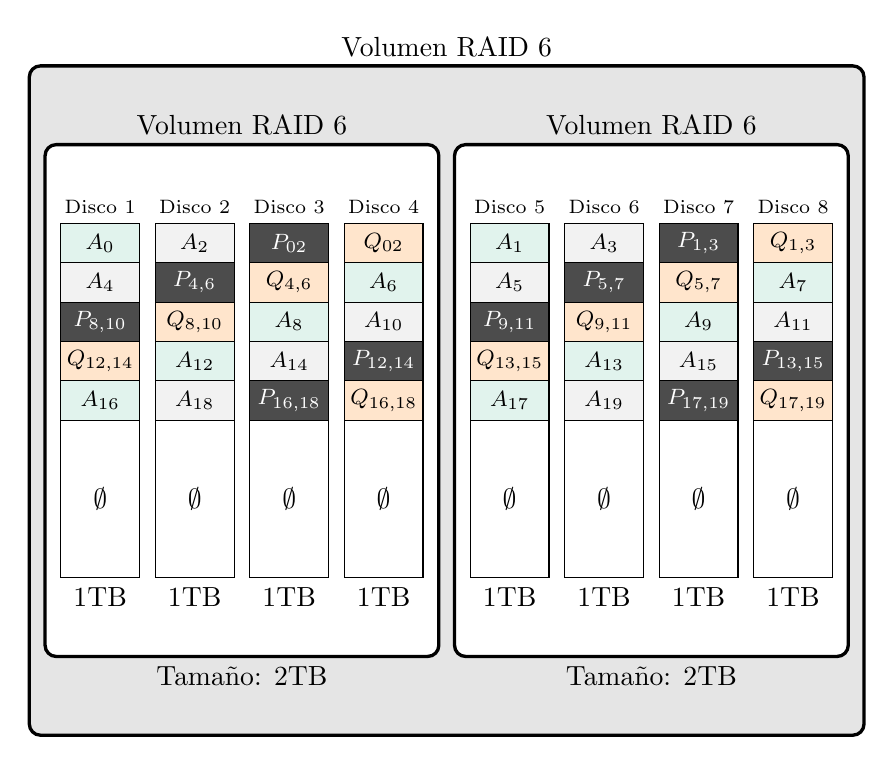
\begin{tikzpicture}
    \draw[very thick,rounded corners,fill=gray!20] (-.4,-4) rectangle (10.2,4.5);
    \node[above] at (4.9,4.5) {Volumen RAID 6};

    \draw[very thick,rounded corners,fill=white] (-.2,-3) rectangle (4.8,3.5);
    \node[above] at (2.3,3.5) {Volumen RAID 6};
    \node[below] at (2.3,-3) {Tamaño: 2TB};

    \draw[very thick,rounded corners,fill=white] (5,-3) rectangle (10,3.5);
    \node[above] at (7.5,3.5) {Volumen RAID 6};
    \node[below] at (7.5,-3) {Tamaño: 2TB};

    \node[above,font=\scriptsize] at (0.5,2.5) {Disco 1};
    \foreach \y\t\c in {
        0/A_{16}/white!95!blue!93!green,
        0.5/Q_{12,14}/orange!20,
        1/\color{white}P_{8,10}/black!70,
        1.5/A_4/gray!10,
        2/A_0/white!95!blue!93!green}{
      \draw[fill=\c,font=\footnotesize] (0,\y) rectangle node{\(\t\)} (1,{0.5+\y});
    }
    \draw (0,0) rectangle node{\(\emptyset\)} (1,-2);
    \node[below] at (0.5,-2) {1TB};

    \node[above,font=\scriptsize] at (1.7,2.5) {Disco 2};
    \foreach \y\t\c in {
        0/A_{18}/gray!10,
        0.5/A_{12}/white!95!blue!93!green,
        1/Q_{8,10}/orange!20,
        1.5/\color{white}P_{4,6}/black!70,
        2/A_2/gray!10}{
      \draw[fill=\c,font=\footnotesize] (1.2,\y) rectangle node{\(\t\)} (2.2,{0.5+\y});
    }
    \draw (1.2,0) rectangle node{\(\emptyset\)} (2.2,-2);
    \node[below] at (1.7,-2) {1TB};

    \node[above,font=\scriptsize] at (2.9,2.5) {Disco 3};
    \foreach \y\t\c in {
        0/\color{white}P_{16,18}/black!70,
        0.5/A_{14}/gray!10,
        1/A_8/white!95!blue!93!green,
        1.5/Q_{4,6}/orange!20,
        2/\color{white}P_{02}/black!70}{
      \draw[fill=\c,font=\footnotesize] (2.4,\y) rectangle node{\(\t\)} (3.4,{0.5+\y});
    }
    \draw (2.4,0) rectangle node{\(\emptyset\)} (3.4,-2);
    \node[below] at (2.9,-2) {1TB};

    \node[above,font=\scriptsize] at (4.1,2.5) {Disco 4};
    \foreach \y\t\c in {
        0/Q_{16,18}/orange!20,
        0.5/\color{white}P_{12,14}/black!70,
        1/A_{10}/gray!10,
        1.5/A_{6}/white!95!blue!93!green,
        2/Q_{02}/orange!20}{
      \draw[fill=\c,font=\footnotesize] (3.6,\y) rectangle node{\(\t\)} (4.6,{0.5+\y});
    }
    \draw (3.6,0) rectangle node{\(\emptyset\)} (4.6,-2);
    \node[below] at (4.1,-2) {1TB};

    % Segundo bloque

    \node[above,font=\scriptsize] at (5.7,2.5) {Disco 5};
    \foreach \y\t\c in {
        0/A_{17}/white!95!blue!93!green,
        0.5/Q_{13,15}/orange!20,
        1/\color{white}P_{9,11}/black!70,
        1.5/A_5/gray!10,
        2/A_1/white!95!blue!93!green}{
      \draw[fill=\c,font=\footnotesize] (5.2,\y) rectangle node{\(\t\)} (6.2,{0.5+\y});
    }
    \draw (5.2,0) rectangle node{\(\emptyset\)} (6.2,-2);
    \node[below] at (5.7,-2) {1TB};

    \node[above,font=\scriptsize] at (6.9,2.5) {Disco 6};
    \foreach \y\t\c in {
        0/A_{19}/gray!10,
        0.5/A_{13}/white!95!blue!93!green,
        1/Q_{9,11}/orange!20,
        1.5/\color{white}P_{5,7}/black!70,
        2/A_3/gray!10}{
      \draw[fill=\c,font=\footnotesize] (6.4,\y) rectangle node{\(\t\)} (7.4,{0.5+\y});
    }
    \draw (6.4,0) rectangle node{\(\emptyset\)} (7.4,-2);
    \node[below] at (6.9,-2) {1TB};

    \node[above,font=\scriptsize] at (8.1,2.5) {Disco 7};
    \foreach \y\t\c in {
        0/\color{white}P_{17,19}/black!70,
        0.5/A_{15}/gray!10,
        1/A_9/white!95!blue!93!green,
        1.5/Q_{5,7}/orange!20,
        2/\color{white}P_{1,3}/black!70}{
      \draw[fill=\c,font=\footnotesize] (7.6,\y) rectangle node{\(\t\)} (8.6,{0.5+\y});
    }
    \draw (7.6,0) rectangle node{\(\emptyset\)} (8.6,-2);
    \node[below] at (8.1,-2) {1TB};

    \node[above,font=\scriptsize] at (9.3,2.5) {Disco 8};
    \foreach \y\t\c in {
        0/Q_{17,19}/orange!20,
        0.5/\color{white}P_{13,15}/black!70,
        1/A_{11}/gray!10,
        1.5/A_7/white!95!blue!93!green,
        2/Q_{1,3}/orange!20}{
      \draw[fill=\c,font=\footnotesize] (8.8,\y) rectangle node{\(\t\)} (9.8,{0.5+\y});
    }
    \draw (8.8,0) rectangle node{\(\emptyset\)} (9.8,-2);
    \node[below] at (9.3,-2) {1TB};

  \end{tikzpicture}
  \caption{Tamaño del volumen de RAID 60: 4TB.}
  \label{fig:raid60}
\end{figure}

Cada RAID 6 mantiene su propia doble paridad y se presenta al RAID 0 superior como un único volumen lógico, como se muestra en la figura \ref{fig:raid60}.

\paragraph{Características}
\begin{itemize}
  \item Combina el alto rendimiento del striping (RAID 0) con la alta tolerancia a fallos de RAID 6.
  \item Requiere al menos ocho discos (dos grupos RAID 6 de cuatro discos cada uno).
  \item La capacidad útil es la suma de las capacidades útiles de cada RAID 6.
\end{itemize}

\paragraph{Tolerancia a fallos}

Cada subarreglo RAID 6 puede soportar la falla simultánea de hasta dos discos.

En consecuencia, un RAID 60 puede tolerar múltiples fallas, siempre que ningún grupo RAID 6 pierda más de dos discos.

Por ejemplo, con dos grupos RAID 6:
\begin{itemize}
  \item Pueden fallar dos discos del primer grupo y dos del segundo grupo.
  \item Puede fallar un disco en un grupo y dos en el otro.
  \item Si fallan tres discos dentro del mismo grupo RAID 6, ese grupo deja de funcionar y, debido a que el RAID 0 depende de todos los grupos, se pierde el volumen completo.
\end{itemize}
En general, el número total de discos que pueden fallar depende de cómo se distribuyan las fallas entre los distintos subarreglos.

RAID 60 está orientado a sistemas de almacenamiento de gran capacidad donde se busca una alta tolerancia a fallos sin sacrificar tanto espacio como en RAID 10. Comparado con RAID 50, prioriza una mayor redundancia a costa de reducir la capacidad útil y el rendimiento de escritura, ofreciendo un excelente equilibrio entre disponibilidad y aprovechamiento del almacenamiento.

